\chapter{Platform as a Service with Openshift}
\label{cha:paas}
Platform as a Service (PaaS) ...

\section{The need for Platform as a Service}
\label{sec:paas-need-for-paas}
As mentioned in Section \vref{sec:caas-kubernetes-worker}, there are some use cases where Kubernetes or in particular CaaS is not suitable anymore. CaaS is suitable if its used by developers, but not for persons without any deep knowledge of Docker and Kubernetes. This is where PaaS platforms come into place, which provide a web console and a template mechanism, which can be used by non-developers. Developers specify templates for the provided services which contains all technical parts of a service infrastructure and non-developers provide values for the exposed parameters which are non-technical, and the PaaS platform instantiates the template and deploys the service infrastructure automatically. \\

Enterprises can profit from PaaS platforms by defining templates for services they provide for their departments, partners or customers, who can create an instance of a provided service on demand, and destroy it if not needed anymore. PaaS platforms provide a self service console, where services can be created, managed and destroyed effortlessly without the need to understand the underlying technology. The self service console could be implemented by enterprises for their use cases, where the self service console interacts with PaaS via its exposed API. \\

PaaS platforms like Openshift usually provide an integration in a Continuous Integration / Continuous Deployment (CI/CD) workflow, which allows to automatically build and deploy new service releases on the PaaS platform automatically via web hooks. Therefore, the PaaS platforms are integrated in the whole software life cycle. This decreases the effort of the developers to interact with the cloud platform and provide additional automation.

\section{Openshift}
\label{sec:paas-kubernetes}
Openshift is a open source PaaS platform, which uses Docker and Kubernetes for the Docker Container orchestration. Openshift is designed as a client server architecture and a master slave architecture. One Openshift cluster can contain multiple Kubernetes clusters which are managed by the Openshift Master-Node which is discussed in Section \vref{sec:paas-openshift-master}. Openshift organizes the Kubernetes namespaces in so called projects, which place all defined resources in a Kubernetes namespace, and which are isolated form each other. Kubernetes organizes the resources in namespaces but does not provide any security mechanism for isolating those namespaces. Kubernetes also provides no monitoring tooling and web console for managing its resources. The Figure \vref{fig:paas-openshift-project-architecture} illustrates the Openshift Project-Architecture, its contained Openshift Objects, Kubernetes objects and their dependency to each other.

\begin{figure}[htbp]
	\centering
	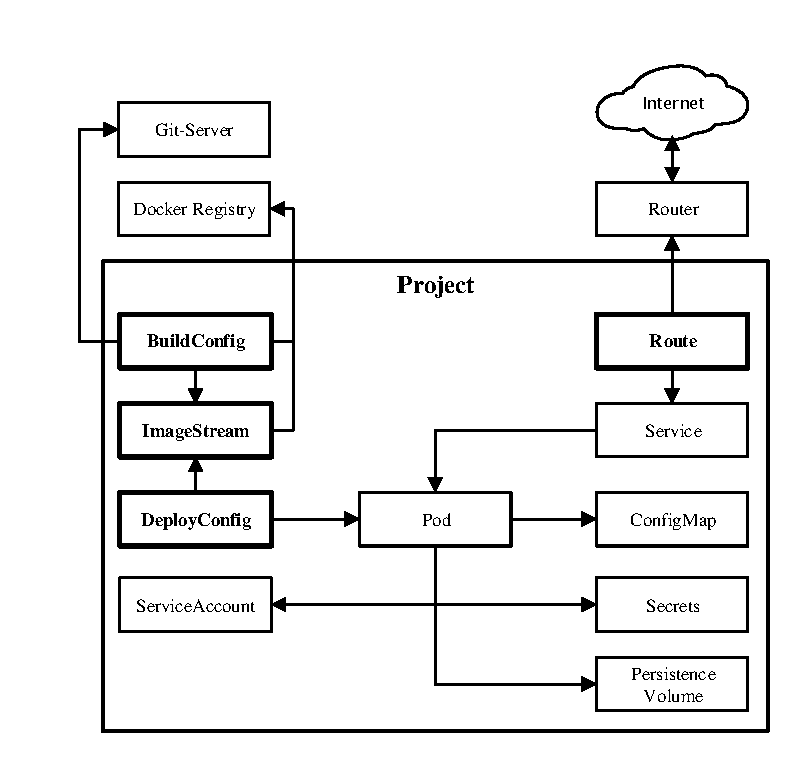
\includegraphics[scale=1]{images/openshift-project-architecture.pdf}
	\caption{Architecture of a Openshift Project}
	\label{fig:paas-openshift-project-architecture}
\end{figure} 
The Openshift Objects, which are contained in an Openshift Project are briefly discussed in the following Section \vref{sec:paas-openshift-objects}.

\subsection{Openshift Objects}
\label{sec:paas-openshift-objects}
Openshift Objects are persistent objects in the Openshift System, and the Openshift Objects describe the state of the Openshift Cluster. This behavior has been inherited from the underlying used Kubernetes System as discussed in Section \vref{sec:caas-kubernetes-objects}. The following sections briefly introduce the Openshift Objects which enhance the Kubernetes System. 

\mysubsubsection{Build Configuration}
The Build Configuration specifies the way how a Docker Image is built on the Openshift platform. The built Docker Image is pushed the Openshift internal Docker Registry. Openshift Build Configurations support the following listed strategies \cite{OpenshiftBuildAndImageStreams2018, S2I2018}.
\begin{itemize}
	\item The \emph{Source-to-Image (S2I)} strategy is the build strategy which builds a Docker Image from source code.
	\item The \emph{Docker} strategy is the build strategy which builds a Docker Image from a Dockerfile.
	\item The \emph{Custom} strategy is the build strategy which build a Docker Image with a custom implemented build mechanism.
	\item The \emph{Pipeline} strategy is the build strategy which performs a Jenkins pipeline build on a Jenkins build server.
\end{itemize}
The necessary resources for the particular build strategy are provided via a git repository, and a Build Configuration can be triggered by an external service such as Github via a web hook. 

\mysubsubsection{Deployment Configuration}
A Deployment Configuration specifies how a deployment unit has to be performed. A Deployment Configuration allow to specify the Kubernetes life cycle hooks pre-hook or post-hook, which are used to configure the deployed Pod before its process has started (pre-hook) or after its process has started and is ready (post-hook). Deployment Configurations support the following deployment strategies.
\begin{itemize}
	\item The \emph{Rolling} strategy is the deployment strategy which waits for the new deployment to be ready before the old deployment gets removed.
	\item The \emph{Recreate} strategy is the deployment strategy which removes the old deployment when the new deployment gets started.
	\item The \emph{Custom} strategy is the deployment strategy which performs the deployment by a custom implementation.
\end{itemize}


\mysubsubsection{Route}
\mysubsubsection{Service}
\mysubsubsection{Docker Registry}

\newpage 

\subsection{Openshift and Kubernetes}
\label{sec:paas-openshift-and-kubernetes}

\begin{figure}[htbp]
	\centering
	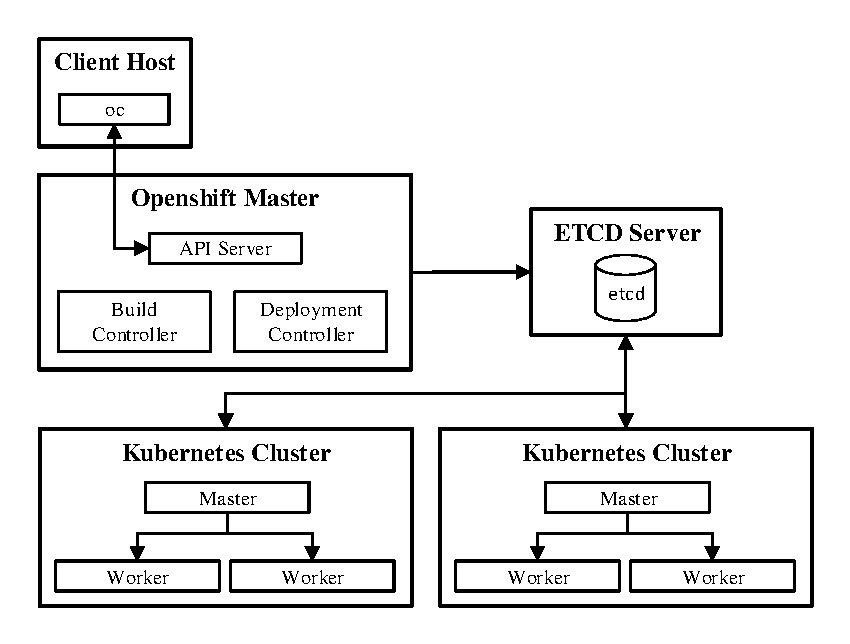
\includegraphics[scale=1]{images/openshift-kubernetes-cluster-architecture.pdf}
	\caption{Architecture of a Openshift-Kubernetes Cluster}
	\label{fig:paas-openshift-kubernetes-cluster-architecture}
\end{figure} 


\subsection{Openshift Master}
\label{sec:paas-openshift-master}